\documentclass[english]{lni}

\IfFileExists{latin1.sty}{\usepackage{latin1}}{\usepackage{isolatin1}}

\usepackage{graphicx}

\author{Alexander Gessler, Simon Hanna, Ashley Marie Smith\\Universit�t Stuttgart, Institute for Parallel and Distributed Systems \\ 
\{gessleah, hannasn, smithae\} @studi.informatik.uni-stuttgart.de}
\title{Scaling in a Distributed Spatial Cache Overlay\footnote{Based on a student project supervised by Carlos L\"{u}bbe at IPVS, University of Stuttgart}}

\begin{document}
\maketitle

\begin{abstract}
Location-based services for mobile devices are a type of distributed system which utilizes geographic behavior of its users. 
Balancing dynamic query workloads and skewed data remains a problem. 
Scale-in and scale-out are two proposals that temporarily remove or add resources, respectively. 
To characterize situations where scaling is more efficient, 
we implemented a distributed spatial cache overlay for 2D data with the goal of evaluating system performance with and without scaling-out. 
In this paper, we present an experimental setup to benchmark such a system, 
and measurements of relative scalability under different cache overlay sizes, query rates and workload distributions. 
Our results indicate that the system achieves almost linear relative scalability for both uniform and non-uniform query distributions.
\end{abstract}

\section{Introduction and Foundations}
Location-based services (LBS) are data-intensive applications which use the geographic behavior of the user in order to process queries. 
These queries access spatial data, which correspond to physical geographic regions. 
A typical example is a route-planning application for smartphones. 
The user sends an address as a query, and in response to the query, the application delivers data, such as the corresponding portion of the map. 
A fundamental problem of LBS is how to allocate workload in the system, 
so as to guarantee low latency and efficiency in processing these queries. 

In an LBS, both query workloads and data have spatial and temporal aspects, 
which dynamically change and thus require special considerations. 
Query loads can vary depending on time or geographic density of users. 
For example, fewer queries are sent late at night or in rural areas. 
Sometimes many queries request data from one location, for instance when large crowds gather for an event. 
Moreover, the distribution of data can be skewed, i.e. non-uniformly clustered around certain spatial regions, like big cities. 

Given these spatial and temporal characteristics, 
we are interested in minimizing decreases in system performance under such loads or data distribution. 
Much research has focused on load-balancing mechanisms for distributed systems with spatial data.
A common technique is to partition data and then build a network overlay, which dedicates nodes to handle requests for certain partitions \cite{client:wee}.
Other approaches estimate query loads or calculate weights to place more nodes around expected hotspots \cite{grids:scholl}.
Yet it is difficult to predict or respond to changes, such as moving hotspots. 
A more effective approach dedicates nodes in the overlay to cache frequently accessed data; 
this network is referred to as a \emph{distributed spatial cache overlay} \cite{MultiLevel:Lueb2}. 

However, none of the previously mentioned load-balancing approaches in distributed spatial overlays 
can increase throughput beyond what is already the system maximum. 
Thus extreme spikes in query workloads can exceed the system's maximum capabilities. 
Adding and then removing additional resources to the LBS can address these temporary spikes. 
The idea is that the overlay automatically decides when to add or remove nodes, based on self-measured load. 
Removing nodes is referred to as \emph{scaling-in}, whereas adding nodes is referred to as \emph{scaling-out.}  
In the scope of our project, we investigate whether scaling-out mitigates dynamic peaks in a distributed spatial cache overlay. 

\section{Architecture and Methodology}

Our system is inspired by the concepts presented in \cite{MultiLevel:Lueb2}. 
The data region is partitioned into a 2D grid. 
Then a distributed cache overlay is built on top which consists of nodes dedicated to caching data from certain grid partitions. 
Our grid of cache nodes forms a Delaunay triangulation in a 2D metric space. 
A cache node's coordinate is known as it's \emph{cache focus}, which is important when load-balancing or caching data. 
Greedy routing is used to forward queries to a target node; the desired data are within a specified distance to that node's cache focus.
Based on these general principles, we implemented a scaling-out mechanism for the distributed spatial cache overlay in a cluster environment.

Our system architecture, as seen in Figure \ref{arch}, consists of grid of cache nodes that are organized spatially and deployed on a cluster.  
Nodes receive external queries, which they can forward. 
An external GUI launches and shuts the system down. 
The system runs remotely on a cluster of variable size and can test the grid under different load-balancing and scaling mechanisms. Furthermore, we included an administrative node to initialize overlay construction and a basic logging system. 
Our implementation of scaling-out relies on asynchronous message-passing and handshake confirmation between nodes. 
The idea is that when a node's load exceeds a given threshold, 
the node communicates with its neighbors to confirm 
whether the overload can be relieved by adding a new node.

\begin{figure}[!ht]
  \begin{center}
    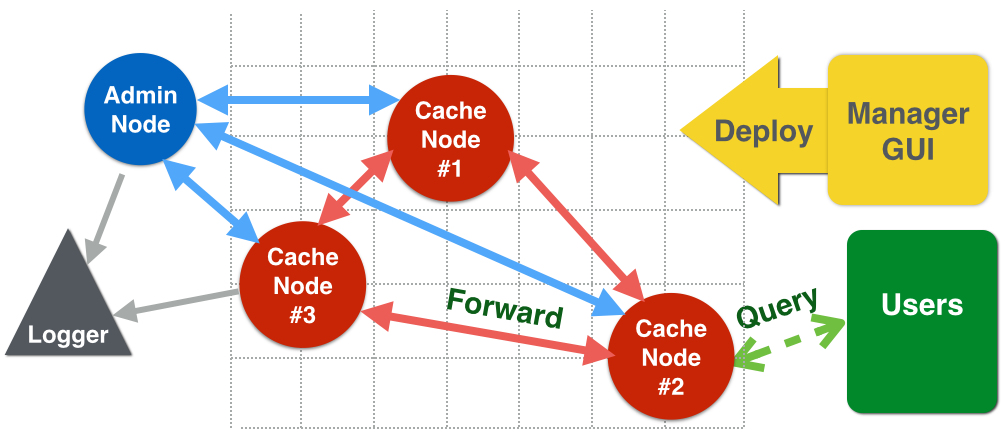
\includegraphics[width=.789\textwidth]{arch2-cropped}
    \caption{\label{arch}System Architecture}
  \end{center}
\end{figure}

The goal of our experiment was to quantify latency under uniform and non-uniform query loads.
In the uniform case, the target coordinates of the queries are distributed uniformly.
However in the non-uniform case, we can simulate the formation of hotspots: 
the target coordinate is obtained by sampling a Gaussian distribution 
with a standard deviation of 0.18 times the area of the data region that is centered around a point in the grid. 
We measured request latency of the cache overlay under three experimental groups
\footnote{We briefly examined the effect of uniform distributions without scaling-out. 
The latency was, as expected, worse than uniform with scaling, but better than our hotspot tests.}
, depending on the type of distribution and presence of scaling-out: 
(1) uniform plus scaling-out, 
(2) hotspot plus scaling-out , 
(3) hotspot.

The distributed spatial cache overlay was launched on a cluster of up to 32 (virtual) machines. 
Our benchmarking program sent each cache node $k$ queries per second. 
This query rate corresponds to about $1000/k$ milliseconds between two successive queries. 
For every experimental group, we ran the benchmark program with query rates of $k = 15$ and $k=20$ 
and a given number of nodes ($n = 8, 12, 16$).
\footnote{The remaining (virtual) machines are used during scaling.}
Each run lasted $10$ seconds, so the total number of queries sent to the grid during each run was $n \cdot 10 \cdot k$. 

\section{Results and Discussion}
	For a given grid size $n$ and query rate $k$, Figures \ref{resultsk15}, \ref{resultsk20} show the median latencies in milliseconds of all queries, 
	according to experimental group.

  \begin{figure}[htb]
    \begin{center}
		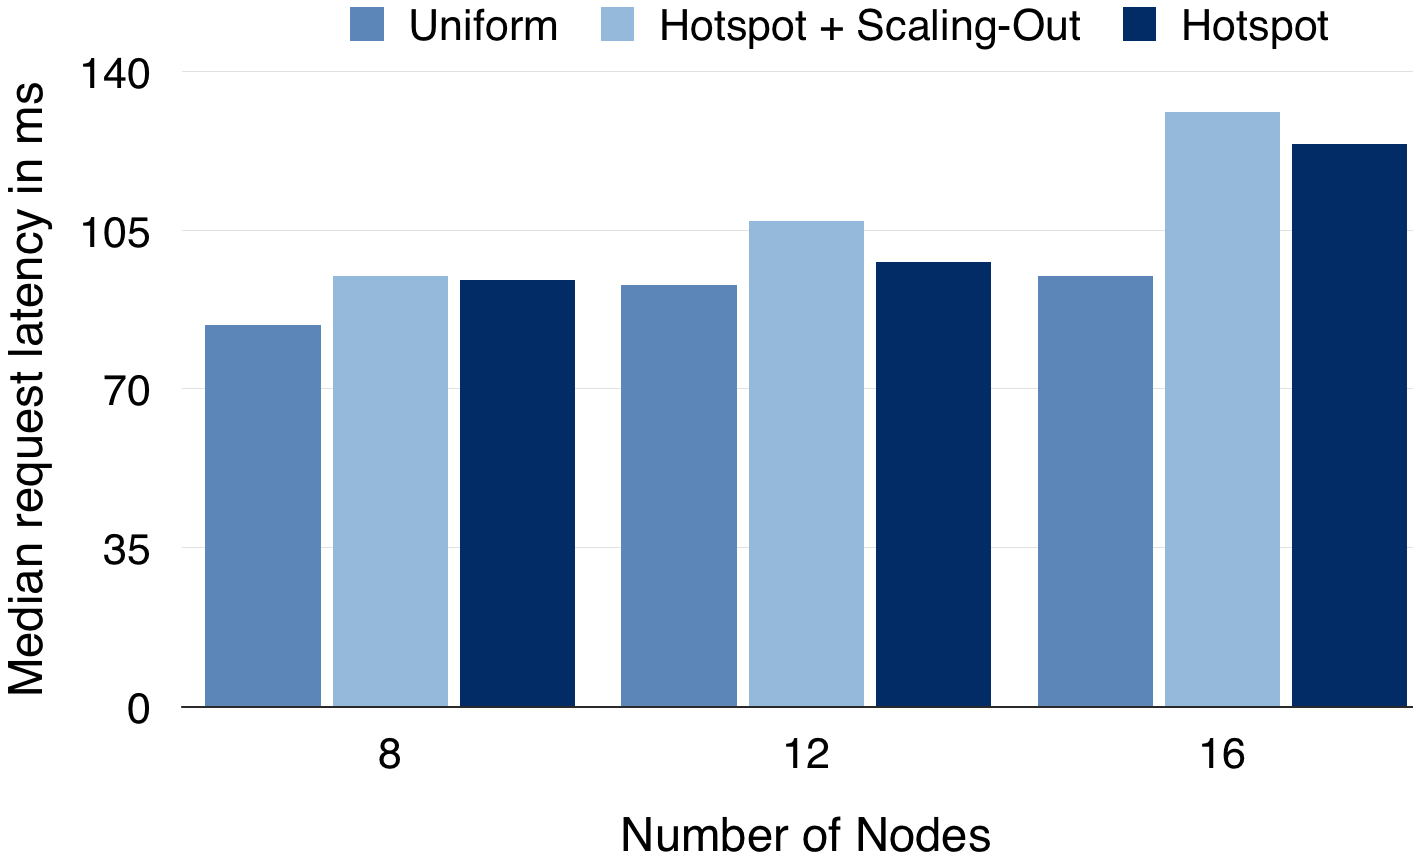
\includegraphics[width=.61\textwidth]{results15}
       \caption{\label{resultsk15} Median Request Latency in $ms$, k=15}
     \end{center}
	\end{figure}

	 \begin{figure}[htb]
    \begin{center}
			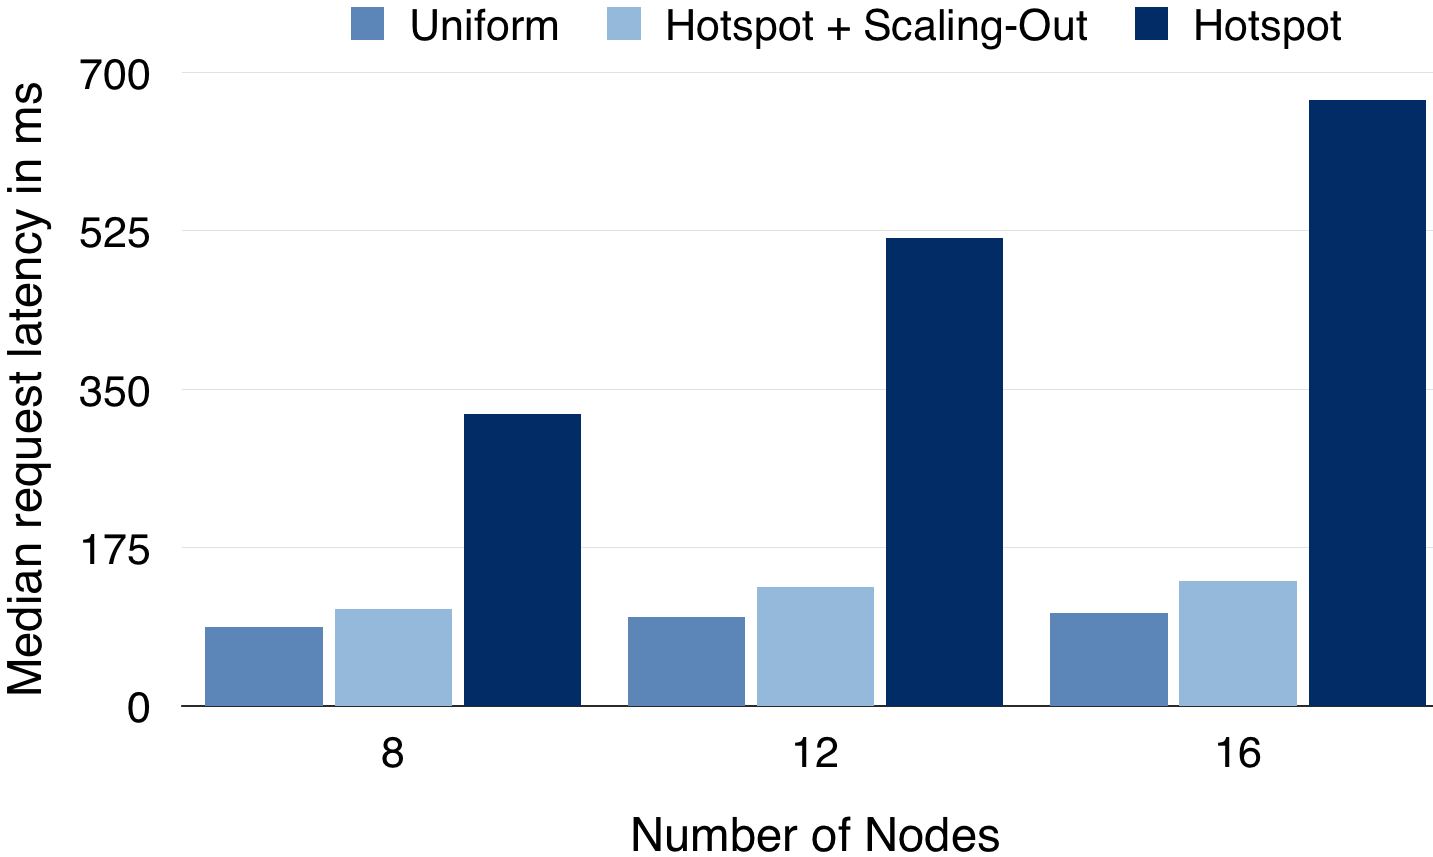
\includegraphics[width=.61\textwidth]{results20}
       \caption{\label{resultsk20} Median Request Latency $ms$, k=20}
     \end{center}
	\end{figure}

We hypothesized that with scaling-out, our system could approximate linear scalability 
in both the uniform and non-uniform cases. 
Our results support our hypothesis. Under the higher request rate $k=20$, 
latency increases markedly for the hotspot group. 
In contrast, the median times for the hotspot (with scaling-out) group when $n=16$ remain within 30 \% of the median latencies 
when $n=8$, although the total number of nodes and therefore the amount of queries being routed to the hotspot has doubled.
			
\section{Conclusion and Future Work}
In our study, we designed, implemented and evaluated a distributed spatial cache overlay 
that is flexible enough to allow implementations of sophisticated load-balancing schemes. 
This cache overlay serves as the basis for further comparisons of various load-balancing mechanisms 
to see whether linear scalability can be achieved. 
We confirmed that non-uniform workloads cause the system's performance and scalability to degrade under higher query rates. 
Using our scaling-out mechanism, we were able to scale the system's performance almost linearly.

Based on our current results, our primary focus will be to implement scaling-in load-balancing 
to handle changes in both global and relative load. 
Since our current implementation exhibits a routing time of $\mathcal O (\sqrt{n})$, 
we propose that our nodes keep skiplist-like connections 
to 2nd or 3rd neighbors as well as local routing shortlists, in order to achieve $\mathcal O (\log n)$ routing.
With local routing shortlists, cache nodes track recent queries which entered the overlay through them, 
along with the cache foci of all the nodes the query visited. 
Nodes could then improve the first routing decision of subsequent queries that enter.

\bibliography{lniguide}
\begin{thebibliography}{1}

\bibitem{grids:scholl}
T.~Scholl, et al. 
``Workload-Aware Data Partitioning in Community-Driven Data Grids."\\
\emph{EDBT}: ACM, 2009.

\bibitem{MultiLevel:Lueb2}
C.~L\"{u}bbe, et al. 
``Holistic load-balancing in a distributed spatial cache."\\
\emph{MDM}: IEEE Computer Society, 2013: pp. 267-270.

\bibitem{client:wee}
S.~Wee and H.~Liu. 
``Client-side load balancer using cloud."\\ 
\emph{SAC}: IEEE Computer Society, 2010, pp. 399-405.

\end{thebibliography}
\end{document}
